%%%%%%%%%%%%%%%%%%%%%%%%%%%%%%%%%%%%%%%%%
% Comprehensive Thesis
%
% Authors:
% Xiaofeng Qian, Son H. Nguyen, Matthew Daddino, Ching Man Wong
% Stevens Institute of Technology
%%%%%%%%%%%%%%%%%%%%%%%%%%%%%%%%%%%%%%%%%

%----------------------------------------------------------------------------------------
%	PACKAGES AND OTHER DOCUMENT CONFIGURATIONS
%----------------------------------------------------------------------------------------

\documentclass[
	a4paper,
	12pt,
	oneside,
]{article}

\usepackage[utf8]{inputenc}
\usepackage[english]{babel}
\usepackage[]{amsthm}
\usepackage[]{amssymb}
\usepackage[]{setspace}
\usepackage[left=1in, right=1in, top=1in, bottom=1in]{geometry}
\usepackage[colorlinks=true, linkcolor=blue, urlcolor=red, citecolor=blue]{hyperref}
\usepackage{xcolor}
\usepackage{soul}
\usepackage{amsmath}
\usepackage{amsfonts}
\usepackage{amssymb}
\usepackage{graphicx}
\usepackage{float}
\usepackage{braket}
\usepackage{gensymb}
\usepackage{booktabs}

\onehalfspacing

%----------------------------------------------------------------------------------------
%	TITLE AND AUTHOR
%----------------------------------------------------------------------------------------

\title{\textbf{Performing Quantum Computation with Classical Optics: \\[0.5em] A Comprehensive Study of the Variational Quantum Eigensolver Implementation via Photonic Systems}}

\author{Son H. Nguyen\textsuperscript{1}, Matthew Daddino\textsuperscript{1}, Ching Man Wong\textsuperscript{1},Xiaofeng Qian\textsuperscript{1}}

\date{\textsuperscript{1}Physics Department, Stevens Institute of Technology, Hoboken, NJ 07030, USA \\[1em] \today}

%----------------------------------------------------------------------------------------

\begin{document}

\maketitle

%----------------------------------------------------------------------------------------
%	ABSTRACT
%----------------------------------------------------------------------------------------

\begin{abstract}
\noindent Quantum computers promise transformative capabilities for molecular simulation and optimization problems, yet practical implementations face significant technological barriers. This thesis demonstrates an alternative approach: implementing quantum algorithms using classical optical systems. We present a comprehensive framework for performing quantum computation through optical components, specifically realizing the Variational Quantum Eigensolver (VQE) algorithm for molecular energy calculations. Our implementation encodes qubits using photonic polarization states and spatial modes, leveraging wave plates (quarter-wave and half-wave), beamsplitters, and dove prisms to construct quantum gates. We detail the theoretical decomposition of the UCCSD (Unitary Coupled Cluster Single and Double excitations) ansatz for the hydrogen molecule, deriving the necessary rotations and entangling operations. The optical realization employs Jones calculus to systematically map quantum gates onto polarization-dependent optical transformations, with Stokes vector measurements enabling quantum state readout. This comprehensive study bridges quantum-algorithm design with optical laboratory realization, demonstrating that quantum algorithms can be executed through photonic platforms as an alternative to superconducting or trapped-ion systems. All derivations, circuit decompositions, and optical implementations are provided in full mathematical detail.
\end{abstract}

\clearpage
\tableofcontents
\clearpage

%----------------------------------------------------------------------------------------
%	1. INTRODUCTION
%----------------------------------------------------------------------------------------

\section{Introduction}

\subsection{Motivation and Background}

Quantum computing offers unprecedented capabilities for solving certain classes of problems that are intractable on classical computers. Among the most promising near-term applications are variational quantum algorithms, which combine classical optimization with quantum simulation. The Variational Quantum Eigensolver (VQE) is one such algorithm, designed to find the ground-state energy of quantum systems—a central problem in quantum chemistry and materials science.

Following the work of O'Malley et al.~\cite{omalley2016scalable}, we begin our analysis with the reduced two-qubit electronic Hamiltonian for molecular hydrogen:
\begin{equation}
\hat{H} = g_0 \mathbb{I} + g_1 Z_0 + g_2 Z_1 + g_3 Z_0 Z_1 + g_4 Y_0 Y_1 + g_5 X_0 X_1,
\label{eq:omalley_hamiltonian}
\end{equation}
where $X_i$, $Y_i$, and $Z_i$ are Pauli operators acting on qubit $i$, and the coefficients $g_k$ depend on molecular geometry (in particular, bond length). This compact form captures the essential electronic structure terms needed for ground-state estimation in a near-term quantum setting.

The individual Pauli matrices are defined as:
\[
X = \begin{bmatrix}
	0 & 1 \\
	1 & 0
\end{bmatrix}, \quad
\mathbb{I} = \begin{bmatrix}
	1 & 0 \\
	0 & 1
\end{bmatrix}, \quad
Y = \begin{bmatrix}
	0 & -i \\
	i & 0
\end{bmatrix}, \quad
Z = \begin{bmatrix}
	1 & 0 \\
	0 & -1
\end{bmatrix}
\]

The two-qubit Hamiltonian matrix representation is:
\[
H = \begin{bmatrix}
	g_0 + g_1 + g_2 + g_3 & 0 & 0 & g_5 - g_4 \\
	0 & g_0 + g_1 - g_2 - g_3 & g_5 + g_4 & 0 \\
	0 & g_5 + g_4 & g_0 - g_1 + g_2 - g_3 & 0 \\
	g_5 - g_4 & 0 & 0 & g_0 - g_1 - g_2 + g_3
\end{bmatrix}
\]

\subsection{The Variational Quantum Eigensolver}

Estimating the minimum eigenvalue of Eq.~\ref{eq:omalley_hamiltonian} is the central task of the Variational Quantum Eigensolver (VQE). The algorithm proceeds as follows:
\begin{enumerate}
	\item Prepare a parameterized trial state using a quantum circuit (the \textit{ansatz})
	\item Measure the expectation value $\langle \psi(\boldsymbol{\theta}) | \hat{H} | \psi(\boldsymbol{\theta}) \rangle$
	\item Use classical optimization to update parameters $\boldsymbol{\theta}$ to minimize the energy
	\item Repeat until convergence
\end{enumerate}

In the standard digital model, this procedure is implemented with a reference state preparation, single-qubit rotations, and entangling gates that realize a UCC-inspired ansatz for H$_2$.

\subsection{Classical Optics as a Quantum Simulator}

Rather than implementing VQE on a superconducting qubit or trapped-ion platform, this thesis investigates how the same quantum-information workflow can be implemented using classical optical systems. The key insight is that quantum information can be encoded and manipulated using photonic degrees of freedom, specifically polarization and spatial mode. We map:
\begin{itemize}
	\item Qubit states to photonic polarization states (horizontal $\ket{0}_p$, vertical $\ket{1}_p$) and spatial modes
	\item Unitary gate operations to physically realizable optical transformations built from:
	\begin{itemize}
		\item Quarter-wave plates (QWP) for polarization rotation
		\item Half-wave plates (HWP) for polarization transformation
		\item Beam splitters (BS) for mode coupling
		\item Dove prisms (DP) for spatial mode rotation
		\item Polarizing beam splitters (PBS) for polarization-dependent routing
	\end{itemize}
	\item Quantum measurements to Stokes parameter measurements
\end{itemize}

Jones-matrix and Stokes-parameter formalisms are used to connect the theoretical circuit operations to measurable optical quantities.

\subsection{Thesis Scope and Organization}

The goal of this thesis is not to claim a universal quantum speedup with classical hardware, but to construct a physically transparent and experimentally accessible platform for studying quantum-circuit structure, variational optimization behavior, and measurement strategies motivated by quantum chemistry. By grounding the study in the O'Malley Hamiltonian and the H$_2$ VQE benchmark, we provide a concrete bridge between quantum-algorithm design and optical laboratory realization.

The thesis is organized as follows:
\begin{enumerate}
	\item \textbf{Section 2:} Optical components and their Jones-matrix representations
	\item \textbf{Section 3:} Qubit encoding in photonic systems (polarization and spatial modes)
	\item \textbf{Section 4:} Quantum gate realization with optical components
	\item \textbf{Section 5:} UCCSD ansatz decomposition and circuit preparation
	\item \textbf{Section 6:} Detailed state evolution through the quantum circuit
	\item \textbf{Section 7:} Measurement and readout via Stokes vectors
	\item \textbf{Section 8:} Conclusions and future directions
\end{enumerate}

%----------------------------------------------------------------------------------------
%	2. OPTICAL COMPONENTS
%----------------------------------------------------------------------------------------

\section{Optical Components and Jones Matrices}

\subsection{Overview of Components}

The implementation of quantum gates through optical systems relies on a suite of well-characterized optical components. Each component is described by its Jones matrix, which describes how the component transforms the polarization state of light. In this section, we provide a detailed account of the optical components used in our VQE implementation.

\subsection{Wave Plates}

\subsubsection{Quarter-Wave Plate (QWP)}

A quarter-wave plate introduces a phase retardation of $\pi/2$ between orthogonal polarization components. The Jones matrix for a QWP with fast axis at angle $\theta$ with respect to the horizontal axis is:
\begin{equation}
\text{QWP}(\theta) = e^{\frac{-i\pi}{4}} \begin{bmatrix}
	\cos^2(\theta) + i\sin^2(\theta) & (1-i)\sin(\theta)\cos(\theta) \\
	(1-i)\sin(\theta)\cos(\theta) & \sin^2(\theta) + i\cos^2(\theta)
\end{bmatrix}
\end{equation}

For specific orientations:

\textbf{QWP with vertical fast axis:}
\begin{equation}
\text{QWP}_v = e^{\frac{i\pi}{4}} \begin{bmatrix}
	1 & 0 \\
	0 & -i
\end{bmatrix}
\end{equation}

\textbf{QWP with horizontal fast axis:}
\begin{equation}
\text{QWP}_h = e^{\frac{-i\pi}{4}} \begin{bmatrix}
	1 & 0 \\
	0 & i
\end{bmatrix}
\end{equation}

\begin{figure}[H]
\centering
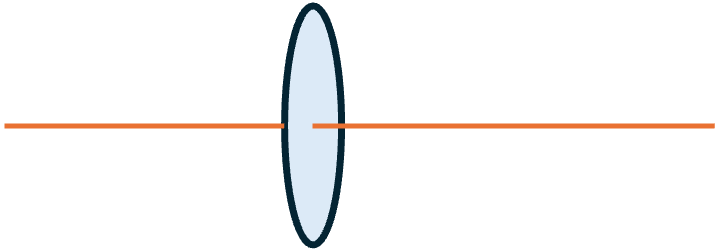
\includegraphics[width=0.25\textwidth]{QWP.png}
\caption{Quarter-wave plate schematic representation.}
\label{fig:qwp}
\end{figure}

\subsubsection{Half-Wave Plate (HWP)}

A half-wave plate introduces a phase retardation of $\pi$ between orthogonal polarization components. The Jones matrix for an HWP with fast axis at angle $\phi$ is:
\begin{equation}
\text{HWP}(\phi) = \begin{bmatrix}
	\cos(2\phi) & \sin(2\phi) \\
	\sin(2\phi) & -\cos(2\phi)
\end{bmatrix}
\end{equation}

\begin{figure}[H]
\centering
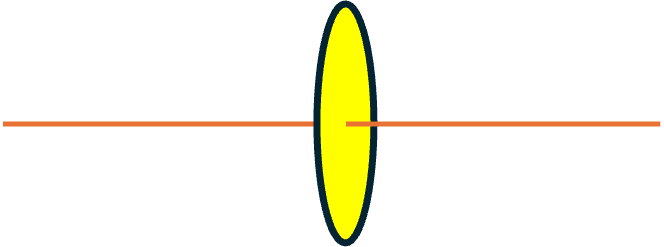
\includegraphics[width=0.25\textwidth]{HWP.png}
\caption{Half-wave plate schematic representation.}
\label{fig:hwp}
\end{figure}

\subsection{Mode-Coupling Devices}

\subsubsection{Beam Splitter (BS)}

A beam splitter couples two spatial modes, directing portion of the light to each output. The transmittance and reflectance determine the coupling strength.

\begin{figure}[H]
\centering
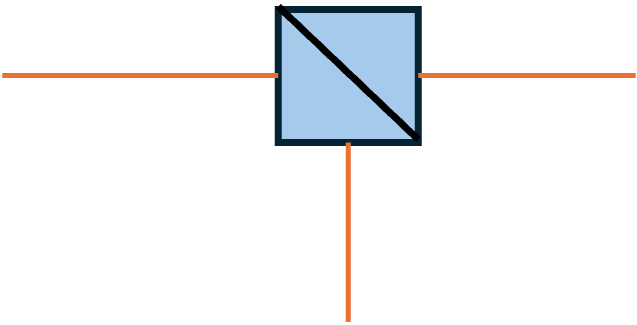
\includegraphics[width=0.25\textwidth]{BS.png}
\caption{Beam splitter schematic representation.}
\label{fig:bs}
\end{figure}

\subsubsection{Polarizing Beam Splitter (PBS)}

A polarizing beam splitter performs mode coupling that is dependent on polarization. Horizontally polarized light is typically transmitted, while vertically polarized light is reflected.

\begin{figure}[H]
\centering
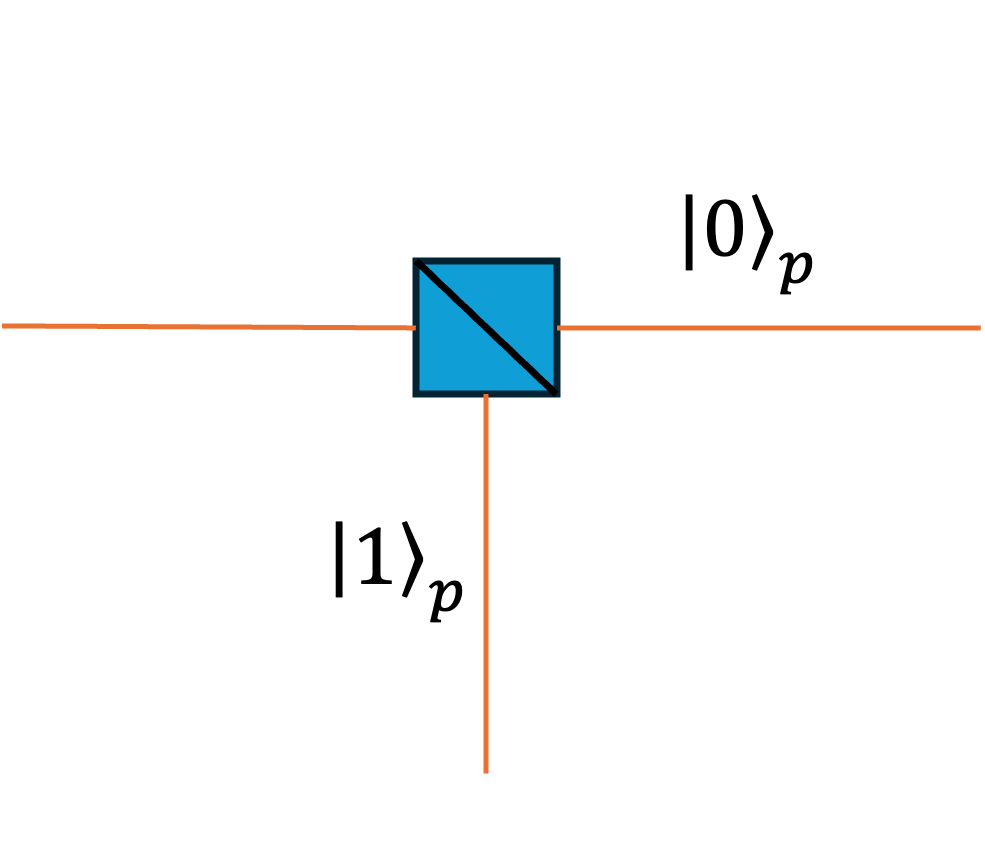
\includegraphics[width=0.35\textwidth]{PBS.png}
\caption{Polarizing beam splitter schematic representation.}
\label{fig:pbs}
\end{figure}

\subsubsection{Dove Prism (DP)}

A dove prism rotates the spatial mode by acting as a rotation operator. The rotation angle $\omega$ determines how the spatial modes are rotated:
\begin{equation}
\text{DP}(\omega) = \begin{bmatrix}
	\cos(\omega) & -\sin(\omega) \\
	\sin(\omega) & \cos(\omega)
\end{bmatrix}
\end{equation}

\begin{figure}[H]
\centering
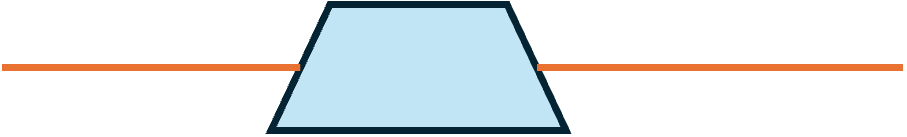
\includegraphics[width=0.3\textwidth]{DP.png}
\caption{Dove prism schematic representation.}
\label{fig:dp}
\end{figure}

%----------------------------------------------------------------------------------------
%	3. QUBIT ENCODING AND INITIAL STATE
%----------------------------------------------------------------------------------------

\section{Qubit Encoding in Photonic Systems}

\subsection{Polarization and Spatial Modes}

In our implementation, we encode quantum information using two degrees of freedom of a photon:
\begin{itemize}
	\item \textbf{First qubit ($q_0$):} Horizontal ($\ket{0}_p$) and vertical ($\ket{1}_p$) polarization states
	\item \textbf{Second qubit ($q_1$):} Spatial modes ``01'' ($\ket{0}_s$) and ``10'' ($\ket{1}_s$)
\end{itemize}

This hybrid encoding allows us to implement two-qubit operations while using a single photon.

\subsection{Basis States and Superpositions}

The computational basis states are:
\begin{align}
\ket{0} &= \text{Spatial Mode 10 and Horizontal Polarization} = \ket{0}_s \otimes \ket{0}_p \\
\ket{1} &= \text{Spatial Mode 01 and Vertical Polarization} = \ket{1}_s \otimes \ket{1}_p
\end{align}

Superposition states on the Bloch/Poincaré sphere include:
\begin{align}
\frac{\ket{0}-i\ket{1}}{\sqrt{2}} &= \text{South Pole of Poincaré Sphere (Left-circular Polarization)} \\
\frac{\ket{0}+i\ket{1}}{\sqrt{2}} &= \text{North Pole of Poincaré Sphere (Right-circular Polarization)} \\
\ket{+} &= \frac{\ket{0}+\ket{1}}{\sqrt{2}} = \text{Diagonal Polarization} \\
\ket{-} &= \frac{\ket{0}-\ket{1}}{\sqrt{2}} = \text{Anti-diagonal Polarization}
\end{align}

\begin{figure}[H]
\centering
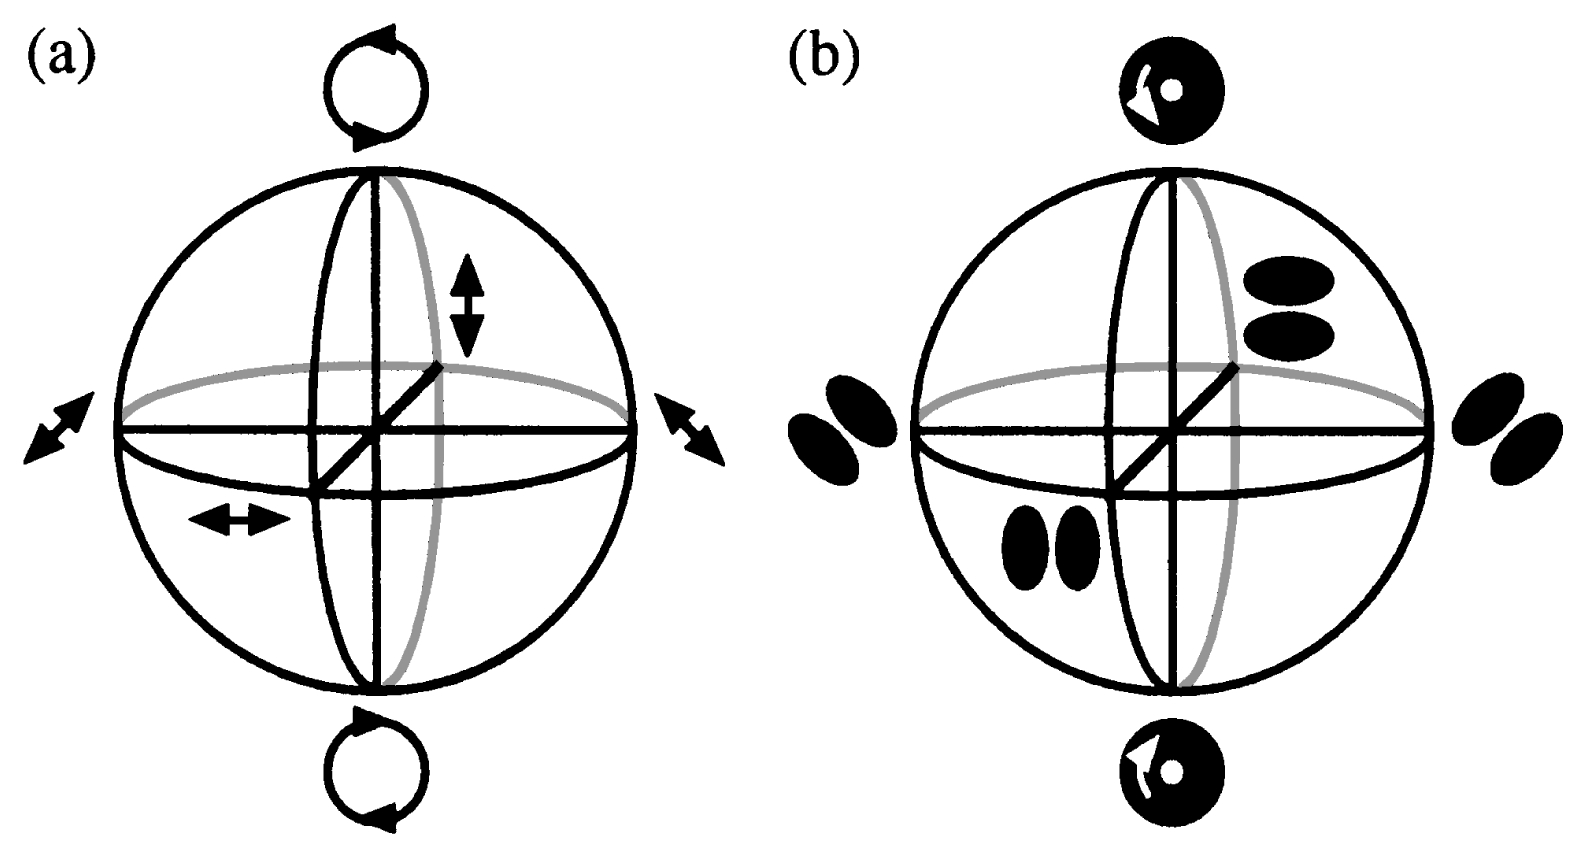
\includegraphics[width=0.4\textwidth]{poincare.jpeg}
\caption{Poincaré sphere showing various polarization states and their relationships.}
\label{fig:poincare}
\end{figure}

\subsection{Initial State Preparation}

The initial state for the VQE algorithm is prepared as:
\[
\ket{\psi_0} = \ket{0}_p \otimes \ket{0}_s = \ket{00}
\]

For the hydrogen molecule, we want to represent the reference state as $\ket{10}$ (one electron in each spatial orbital). This is prepared from $\ket{00}$ by applying an $X$ gate to the first qubit:
\[
\ket{\psi_{\text{ref}}} = (X \otimes I) \ket{00} = \ket{10}
\]

In matrix form:
\[
(X \otimes I) \cdot \begin{bmatrix}1 \\ 0 \\ 0 \\ 0\end{bmatrix} = \begin{bmatrix}0 \\ 0 \\ 1 \\ 0\end{bmatrix} = \ket{10}
\]

\begin{figure}[H]
\centering
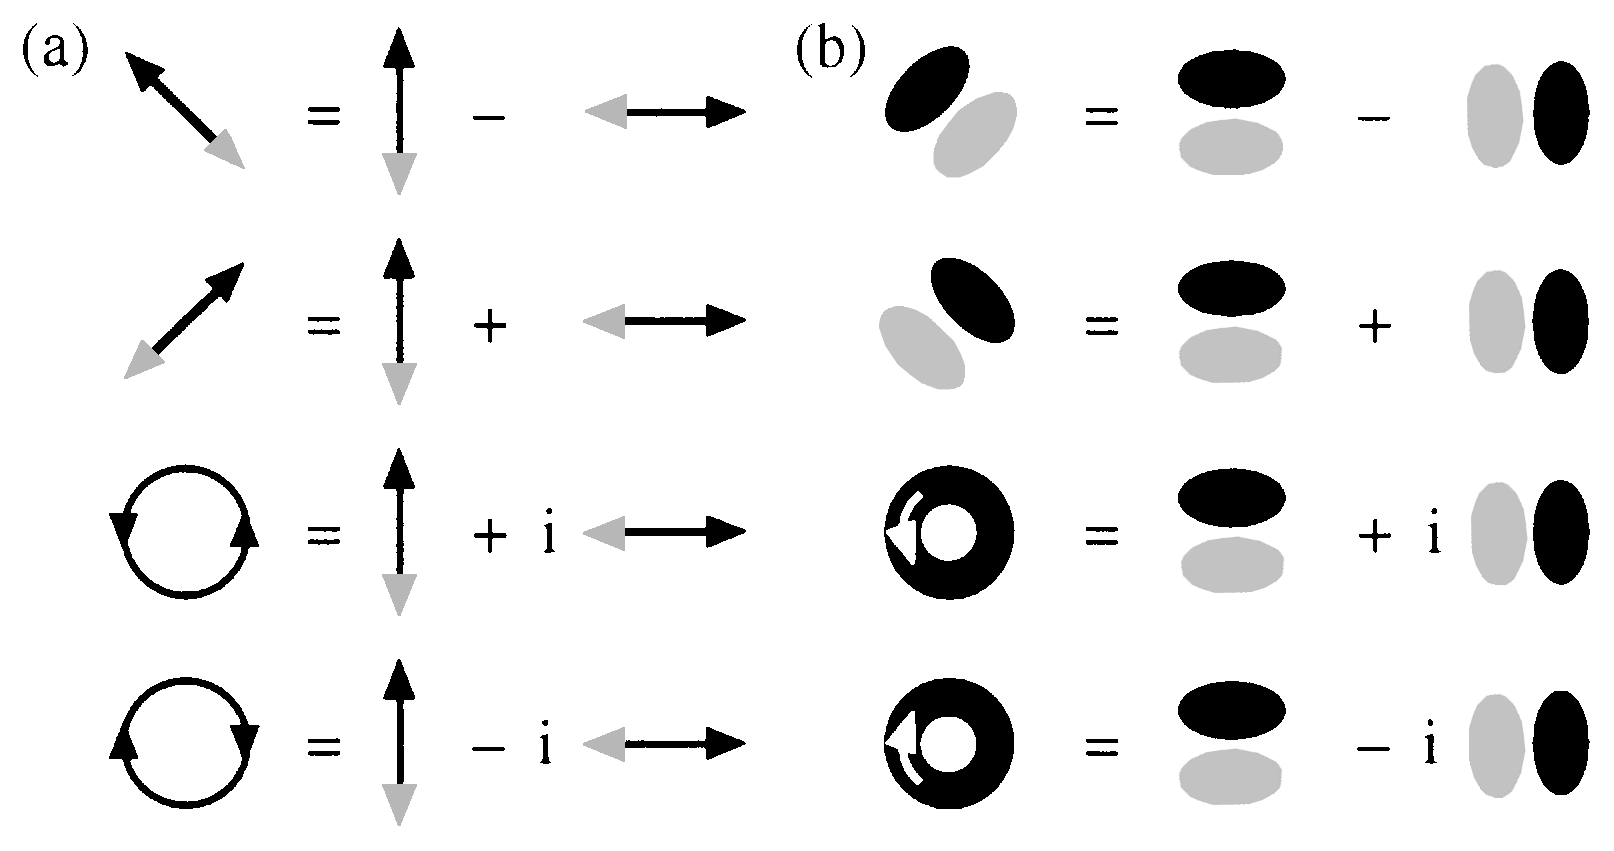
\includegraphics[width=0.4\textwidth]{phaseShift.jpeg}
\caption{Geometric phase shift in the optical implementation.}
\label{fig:phase-shift}
\end{figure}

%----------------------------------------------------------------------------------------
%	4. QUANTUM GATE REALIZATION
%----------------------------------------------------------------------------------------

\section{Quantum Gate Realization with Optical Components}

\subsection{General Approach}

Each quantum gate can be decomposed into a combination of optical components. The Jones matrix for the composite system is obtained by multiplying the Jones matrices of individual components. By carefully choosing component parameters, we can realize arbitrary single-qubit rotations and two-qubit interactions.

\subsection{Single-Qubit Rotations}

\subsubsection{Rx Gate (Rotation around X-axis)}

The quantum $R_x(\theta)$ gate rotates a qubit around the X-axis:
\begin{equation}
R_x(\theta) = \begin{bmatrix}
	\cos(\frac{\theta}{2}) & -i\sin(\frac{\theta}{2}) \\
	-i\sin(\frac{\theta}{2}) & \cos(\frac{\theta}{2})
\end{bmatrix}
\end{equation}

For the specific case $\theta = \pi/2$:
\begin{equation}
R_x(\frac{\pi}{2}) = \frac{1}{\sqrt{2}} \begin{bmatrix}
	1 & -i \\
	-i & 1
\end{bmatrix}
\end{equation}

Acting on $\ket{0}$:
\begin{equation}
R_x(\frac{\pi}{2}) \ket{0} = \frac{1}{\sqrt{2}} \begin{bmatrix}
	1 \\
	-i
\end{bmatrix} = \frac{\ket{0} - i\ket{1}}{\sqrt{2}}
\end{equation}

\textbf{Optical realization:} The $R_x$ gate can be realized using a quarter-wave plate at $\theta = \pi/4$:
\begin{align}
\text{QWP}(\frac{\pi}{4}) &= \frac{1+i}{2} \begin{bmatrix}
	1 & -i \\
	-i & 1
\end{bmatrix}
\end{align}

When a horizontally polarized photon passes through the QWP at $45°$:
\begin{align}
\text{QWP}(\frac{\pi}{4}) \ket{0}_p &= \frac{1+i}{2} \begin{bmatrix}
	1 \\
	-i
\end{bmatrix} = \frac{1+i}{2} \ket{L}_p
\end{align}

where $\ket{L}_p$ represents left-circular polarization. This creates the desired superposition state with the appropriate phase.

\begin{figure}[H]
\centering
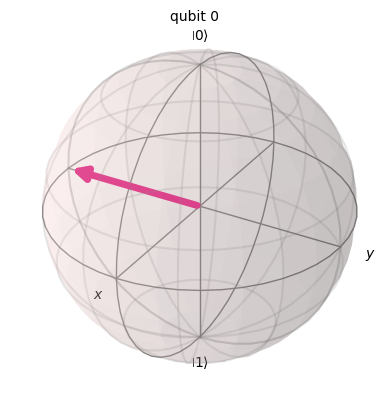
\includegraphics[width=0.4\textwidth]{Rxgatequantum.png}
\caption{Quantum state $\frac{\ket{0}-i\ket{1}}{\sqrt{2}}$ produced by the $R_x(\pi/2)$ gate.}
\label{fig:rx-gate}
\end{figure}

\subsubsection{Time-Dependent Electric Field}

The time-dependent electric field can be extracted from the Jones vector using:
\begin{align}
\vec{E}(t) &= \text{Re}\{\ket{E} e^{-i\omega t}\} \\
\vec{E}_x(t) &= \text{Re}(E_x e^{-i\omega t}) \\
\vec{E}_y(t) &= \text{Re}(E_y e^{-i\omega t})
\end{align}

\begin{figure}[H]
\centering
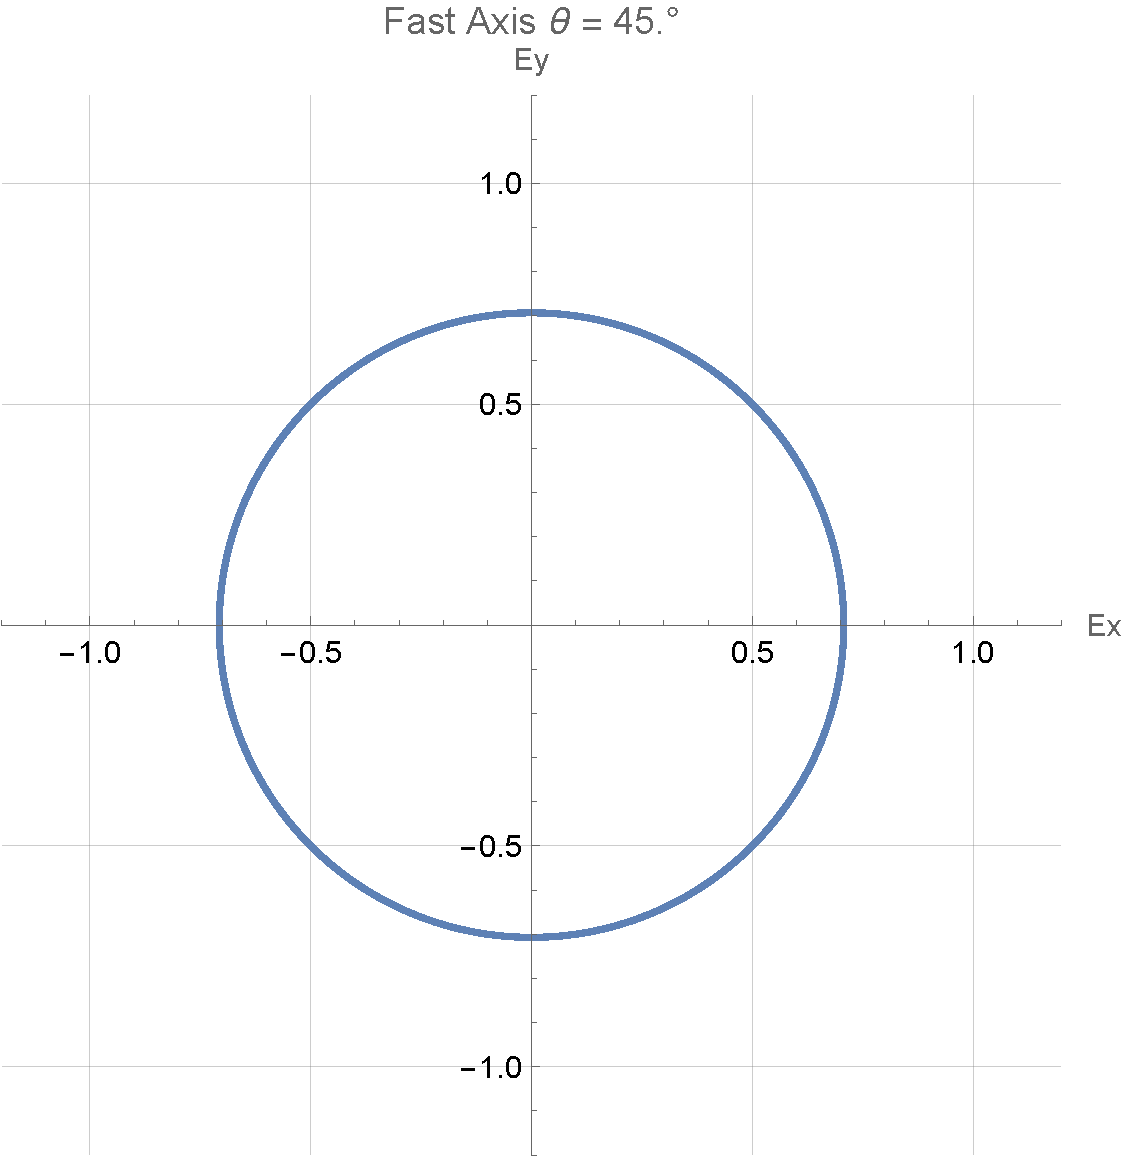
\includegraphics[width=0.4\textwidth]{EfieldRx.pdf}
\caption{Time-dependent electric field components for the $R_x(\pi/2)$ gate output state.}
\label{fig:efield}
\end{figure}

\subsubsection{Rx(\(\pi\)) Gate}

For a $\pi$ rotation:
\begin{equation}
R_x(\pi) = \begin{bmatrix}
	0 & -i \\
	-i & 0
\end{bmatrix} = -i \begin{bmatrix}
	0 & 1 \\
	1 & 0
\end{bmatrix}
\end{equation}

This can be realized by stacking two QWPs appropriately.

\subsection{Two-Qubit Gates}

Two-qubit entangling gates (such as CNOT) are realized through mode-coupling devices that create correlations between the spatial modes and polarization states. The precise implementation involves sequences of beam splitters and wave plates that entangle the two qubits.

%----------------------------------------------------------------------------------------
%	5. UCCSD ANSATZ AND CIRCUIT PREPARATION
%----------------------------------------------------------------------------------------

\section{UCCSD Ansatz Decomposition}

\subsection{Overview of the Ansatz}

The Unitary Coupled Cluster with Singles and Doubles (UCCSD) ansatz is a standard choice for VQE in quantum chemistry. For the hydrogen molecule with two qubits, the ansatz involves:
\begin{enumerate}
	\item Initial state preparation: $\ket{\psi_{\text{ref}}} = \ket{10}$
	\item Parameterized single-qubit rotations
	\item Parameterized entangling gates (CNOT)
	\item Additional single-qubit rotations
	\item Measurement in the computational basis
\end{enumerate}

\subsection{Circuit Structure}

The complete UCCSD circuit for H$_2$ is shown schematically:

\begin{figure}[H]
\centering
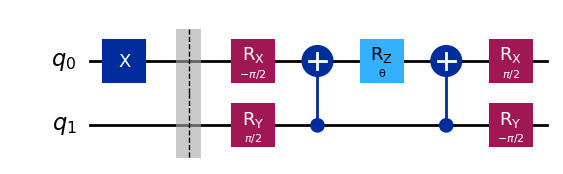
\includegraphics[width=0.85\linewidth]{Circ.png}
\caption{UCCSD ansatz circuit for the hydrogen molecule. The circuit includes initial state preparation, single-qubit rotations (Rx, Ry), entangling CNOT gates, and final measurement.}
\label{fig:uccsd-circuit}
\end{figure}

\subsection{Reference State Preparation}

Starting from the all-zero state $\ket{00}$, we apply an $X$ gate to prepare the reference state $\ket{10}$:
\[
\ket{\psi_{\text{ref}}} = (X \otimes I) \ket{00}
\]

In matrix form:
\[
\begin{bmatrix}
	0 & 1 \\
	1 & 0
\end{bmatrix} \otimes \begin{bmatrix}
	1 & 0 \\
	0 & 1
\end{bmatrix} \cdot \begin{bmatrix}
	1 \\
	0 \\
	0 \\
	0
\end{bmatrix} = \begin{bmatrix}
	0 \\
	0 \\
	1 \\
	0
\end{bmatrix} = \ket{10}
\]

\begin{figure}[H]
\centering
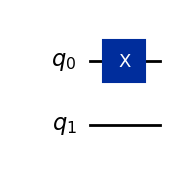
\includegraphics[width=0.2\textwidth]{ref.png}
\caption{Reference state preparation circuit showing the X gate applied to qubit 0.}
\label{fig:ref-state}
\end{figure}

%----------------------------------------------------------------------------------------
%	6. DETAILED STATE EVOLUTION THROUGH THE CIRCUIT
%----------------------------------------------------------------------------------------

\section{State Evolution Through the Ansatz Circuit}

\subsection{Initial State}

The reference state is:
\[
\ket{\psi_0} = \ket{10} = \begin{bmatrix} 0 \\ 0 \\ 1 \\ 0 \end{bmatrix}
\]

\subsection{First Layer: Initial Rotations}

Apply $R_x(-\pi/2) \otimes R_y(\pi/2)$:

\[
R_x(\frac{-\pi}{2}) = \begin{bmatrix}
	\frac{\sqrt{2}}{2} & \frac{i\sqrt{2}}{2} \\
	\frac{i\sqrt{2}}{2} & \frac{\sqrt{2}}{2}
\end{bmatrix}, \quad
R_y(\frac{\pi}{2}) = \begin{bmatrix}
	\frac{\sqrt{2}}{2} & -\frac{\sqrt{2}}{2} \\
	\frac{\sqrt{2}}{2} & \frac{\sqrt{2}}{2}
\end{bmatrix}
\]

The tensor product:
\[
(R_x(\frac{-\pi}{2}) \otimes R_y(\frac{\pi}{2})) = \begin{bmatrix}
	\frac{1}{2} & \frac{-1}{2} & \frac{i}{2} & \frac{-i}{2} \\
	\frac{1}{2} & \frac{1}{2} & \frac{i}{2} & \frac{i}{2} \\
	\frac{i}{2} & \frac{-i}{2} & \frac{1}{2} & \frac{-1}{2} \\
	\frac{i}{2} & \frac{i}{2} & \frac{1}{2} & \frac{1}{2}
\end{bmatrix}
\]

Applied to reference state:
\[
(R_x(\frac{-\pi}{2}) \otimes R_y(\frac{\pi}{2})) \ket{10} = \begin{bmatrix}
	\frac{i}{2} \\
	\frac{i}{2} \\
	\frac{1}{2} \\
	\frac{1}{2}
\end{bmatrix}
\]

\subsection{First CNOT Gate (Entanglement)}

The CNOT gate with qubit 0 as control and qubit 1 as target:
\[
\text{CNOT} = \begin{bmatrix}
	1 & 0 & 0 & 0 \\
	0 & 0 & 0 & 1 \\
	0 & 0 & 1 & 0 \\
	0 & 1 & 0 & 0
\end{bmatrix}
\]

After applying CNOT:
\[
\text{CNOT} \cdot \begin{bmatrix}
	\frac{i}{2} \\
	\frac{i}{2} \\
	\frac{1}{2} \\
	\frac{1}{2}
\end{bmatrix} = \begin{bmatrix}
	\frac{i}{2} \\
	\frac{1}{2} \\
	\frac{1}{2} \\
	\frac{i}{2}
\end{bmatrix}
\]

\subsection{Parameterized $Z_\theta$ Rotation}

The parameterized Z rotation gate:
\[
Z_\theta = \begin{bmatrix}
	e^{-i\theta/2} & 0 \\
	0 & e^{i\theta/2}
\end{bmatrix}
\]

Applied as $(Z_\theta \otimes I)$:
\[
(Z_\theta \otimes I) \cdot \begin{bmatrix}
	\frac{i}{2} \\
	\frac{1}{2} \\
	\frac{1}{2} \\
	\frac{i}{2}
\end{bmatrix} = \begin{bmatrix}
	\frac{\sin(\theta/2)}{2} + i\frac{\cos(\theta/2)}{2} \\
	\frac{\cos(\theta/2)}{2} - i\frac{\sin(\theta/2)}{2} \\
	\frac{\cos(\theta/2)}{2} + i\frac{\sin(\theta/2)}{2} \\
	\frac{-\sin(\theta/2)}{2} + i\frac{\cos(\theta/2)}{2}
\end{bmatrix}
\]

\subsection{Second CNOT Gate}

\[
\text{CNOT} \cdot \begin{bmatrix}
	\frac{\sin(\theta/2)}{2} + i\frac{\cos(\theta/2)}{2} \\
	\frac{\cos(\theta/2)}{2} - i\frac{\sin(\theta/2)}{2} \\
	\frac{\cos(\theta/2)}{2} + i\frac{\sin(\theta/2)}{2} \\
	\frac{-\sin(\theta/2)}{2} + i\frac{\cos(\theta/2)}{2}
\end{bmatrix} = \begin{bmatrix}
	\frac{\sin(\theta/2)}{2} + i\frac{\cos(\theta/2)}{2} \\
	\frac{-\sin(\theta/2)}{2} + i\frac{\cos(\theta/2)}{2} \\
	\frac{\cos(\theta/2)}{2} + i\frac{\sin(\theta/2)}{2} \\
	\frac{\cos(\theta/2)}{2} - i\frac{\sin(\theta/2)}{2}
\end{bmatrix}
\]

\subsection{Final Rotation Layer}

Apply $(R_x(\pi/2) \otimes R_y(-\pi/2))$:

\[
(R_x(\frac{\pi}{2}) \otimes R_y(\frac{-\pi}{2})) = \begin{bmatrix}
	\frac{1}{2} & \frac{1}{2} & \frac{-i}{2} & \frac{-i}{2} \\
	\frac{-1}{2} & \frac{1}{2} & \frac{i}{2} & \frac{-i}{2} \\
	\frac{-i}{2} & \frac{-i}{2} & \frac{1}{2} & \frac{1}{2} \\
	\frac{i}{2} & \frac{-i}{2} & \frac{-1}{2} & \frac{1}{2}
\end{bmatrix}
\]

The final state (after simplification and reordering to match Qiskit convention) is:
\begin{equation}
\ket{\psi(\theta)} = \begin{bmatrix}
	0 \\
	\cos(\theta/2) \\
	-\sin(\theta/2) \\
	0
\end{bmatrix}
\label{eq:ansatz-state}
\end{equation}

This state depends on the variational parameter $\theta$, which is optimized classically to minimize the energy expectation value.

%----------------------------------------------------------------------------------------
%	7. MEASUREMENT AND STOKES VECTOR READOUT
%----------------------------------------------------------------------------------------

\section{Measurement and Stokes Vector Analysis}

\subsection{Jones Vectors and Stokes Vectors}

The Jones vector describes the fully polarized state of light:
\[
\ket{E} = \begin{bmatrix} E_x \\ E_y \end{bmatrix}
\]

The Stokes vector provides a way to measure both polarized and partially polarized light:
\begin{equation}
\vec{S} = \begin{bmatrix}
	I \\
	Q \\
	U \\
	V
\end{bmatrix} = \begin{bmatrix}
	|E_x|^2 + |E_y|^2 \\
	|E_x|^2 - |E_y|^2 \\
	2\text{Re}(E_x E_y^*) \\
	2\text{Im}(E_x E_y^*)
\end{bmatrix}
\label{eq:stokes}
\end{equation}

where:
\begin{itemize}
	\item $I$ is the total intensity
	\item $Q$ describes the preference between horizontal and vertical polarization
	\item $U$ describes the preference between diagonal and anti-diagonal polarization
	\item $V$ describes the preference between right- and left-circular polarization
\end{itemize}

\subsection{Measurement Setup}

The quantum state measurement is performed by:
\begin{enumerate}
	\item Rotating the polarization state using a half-wave plate (HWP) at angle $\phi$
	\item Using a polarizing beam splitter (PBS) to separate horizontal and vertical components
	\item Detecting the number of photons in each output
\end{enumerate}

By rotating the HWP through different angles and measuring the output, we can reconstruct the full Stokes vector and hence determine the quantum state.

\subsection{Optimal Measurement Bases}

To fully characterize the quantum state, measurements must be performed in multiple bases:
\begin{itemize}
	\item \textbf{Computational basis:} Direct PBS measurement (HWP at $0°$)
	\item \textbf{Diagonal basis:} HWP at $22.5°$
	\item \textbf{Circular basis:} QWP at $45°$ followed by PBS
\end{itemize}
The overall optical setup:
\clearpage
\begin{figure}[p]
\vspace*{-1.1cm}
\centering
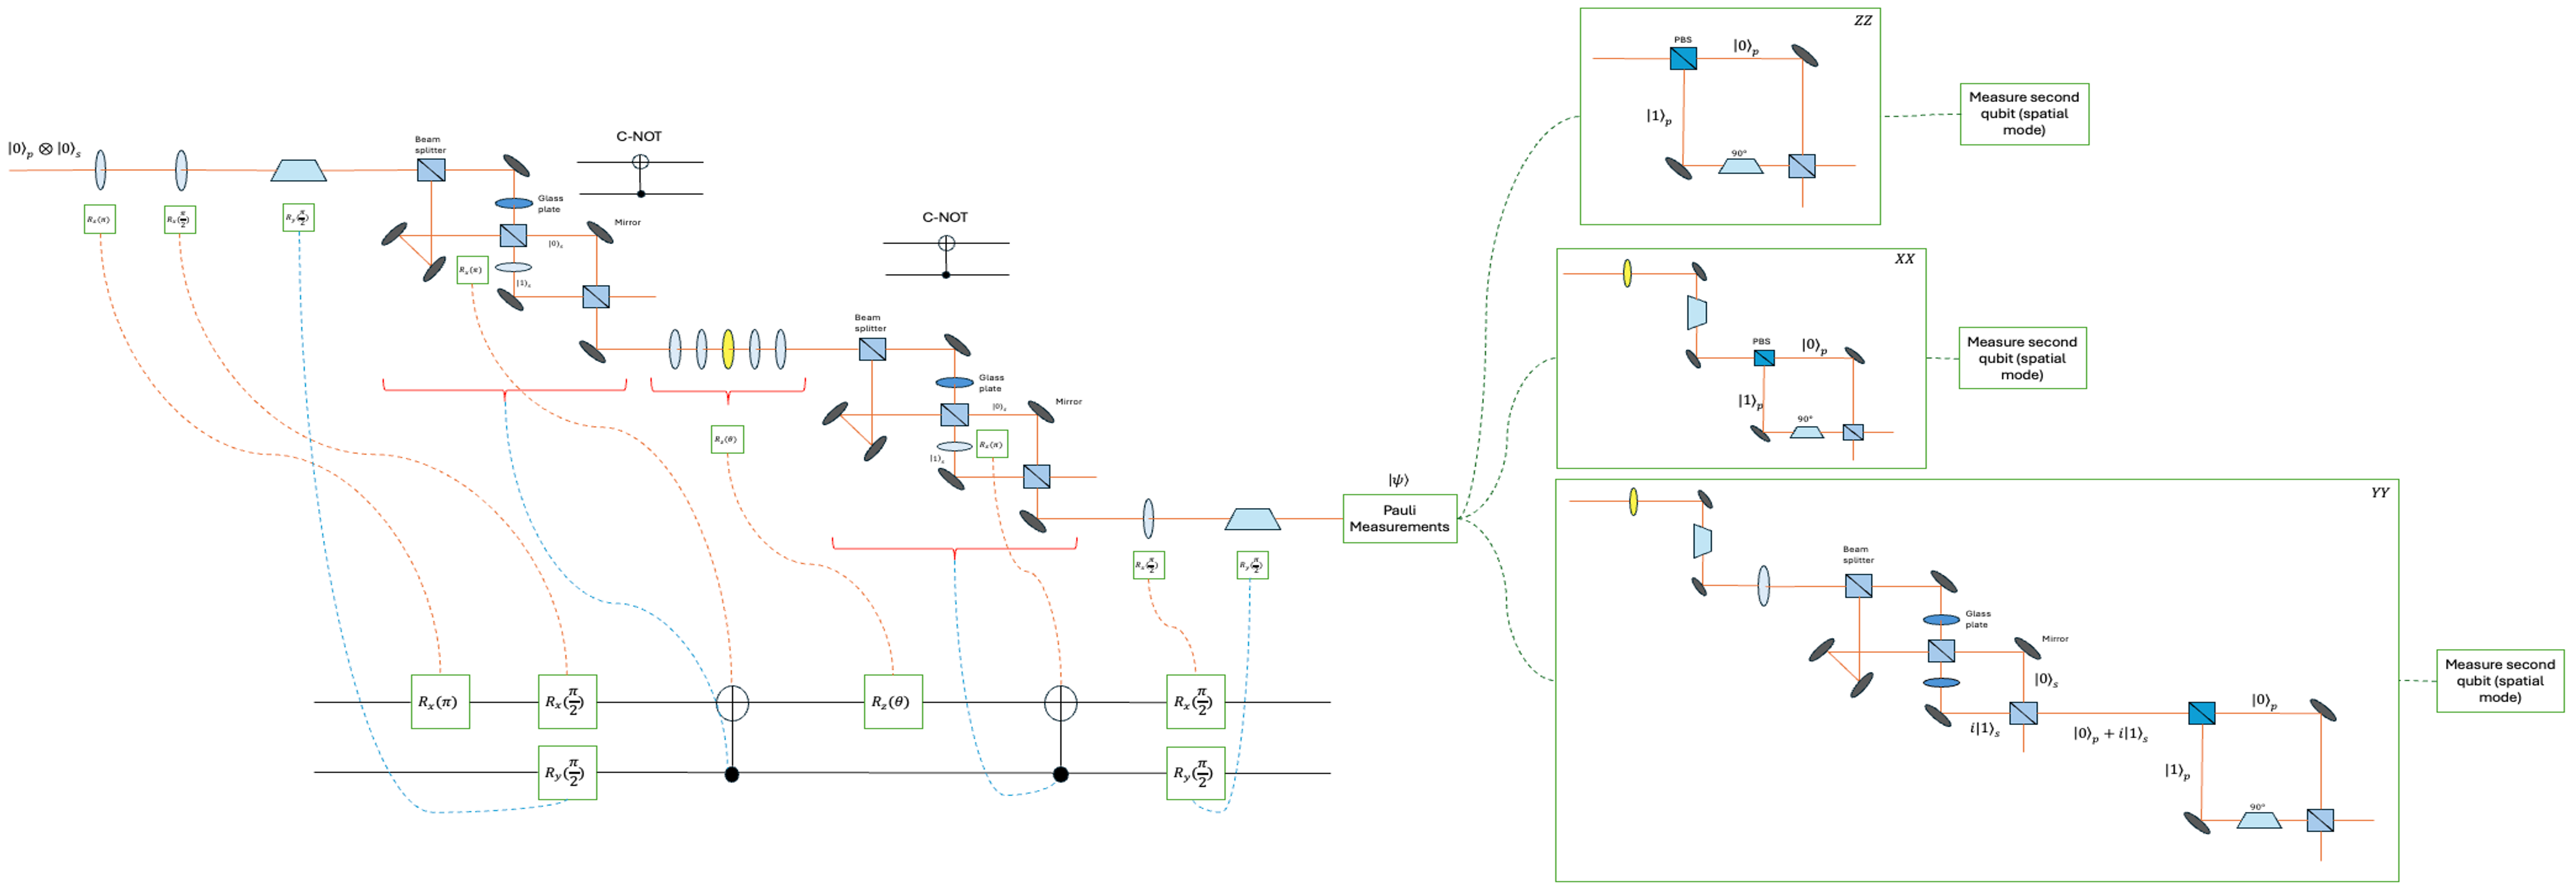
\includegraphics[angle=90, height=1.1\textheight, keepaspectratio]{FullOpticalCirc.png}
\label{fig:full-optical-circuit}
\end{figure}
\clearpage
%----------------------------------------------------------------------------------------
%	8. CONCLUSIONS AND FUTURE DIRECTIONS
%----------------------------------------------------------------------------------------

\section{Conclusions and Future Directions}

\subsection{Summary of Results}

This thesis has presented a comprehensive framework for implementing the Variational Quantum Eigensolver using classical optical systems. We have detailed:

\begin{enumerate}
	\item The complete mapping from quantum gates to optical components
	\item The encoding of two-qubit systems using polarization and spatial modes
	\item The full decomposition of the UCCSD ansatz circuit
	\item The detailed state evolution through the circuit with all intermediate states calculated
	\item The measurement scheme based on Stokes vectors for readout
\end{enumerate}

The key achievement is demonstrating that quantum algorithms can be physically implemented and studied using standard optical laboratory equipment, providing an accessible platform for understanding quantum-circuit behavior and optimization dynamics.

\subsection{Advantages of the Optical Approach}

\begin{itemize}
    \item \textbf{Affordability:} Lower cost compared to traditional quantum computing hardware.
 	\item \textbf{Accessibility:} Uses readily available optical components
	\item \textbf{Transparency:} Direct visualization and measurement of quantum states.
	\item \textbf{Noise robustness:} More robust to certain types of noise.
	\item \textbf{Educational value:} Clear physical realization of quantum concepts
\end{itemize}

\subsection{Limitations and Considerations}

\begin{itemize}
    \item Analogo nature of the implementation may not capture all quantum effects (e.g., true entanglement)
	\item Scaling to larger systems requires more sophisticated mode and polarization encoding
\end{itemize}

\subsection{Future Directions}

Several extensions of this work are promising:

\begin{enumerate}
    \item \textbf{Optimizing the Optical Circuit:} Reduce the number of components and improve stability.
	\item \textbf{Experimental implementation:} Build the optical setup and verify theoretical predictions
	\item \textbf{Optimization studies:} Investigate how the classical optimizer performs with realistic noise
\end{enumerate}

\subsection{Final Remarks}

This comprehensive study bridges the gap between abstract quantum algorithms and concrete physical implementations. By grounding quantum-algorithm design in optical laboratory realization, we provide a platform for both research and education in quantum information processing. The detailed mathematical derivations and circuit decompositions serve as a reference for future work in photonic quantum computing and simulation.

%----------------------------------------------------------------------------------------
%	REFERENCES
%----------------------------------------------------------------------------------------

\clearpage

\begin{thebibliography}{99}

\bibitem{omalley2016scalable}
O'Malley, P. J. J., et al. (2016). Scalable quantum simulation of molecular energies. \textit{Physical Review X}, 6(3), 031007.

\bibitem{kandala2017hardware}
Kandala, A., et al. (2017). Hardware-efficient variational quantum eigensolver for small molecules and quantum magnets. \textit{Nature}, 549(7671), 242-246.

\bibitem{jones1941new}
Jones, R. C. (1941). A new calculus for the treatment of optical systems. \textit{Journal of the Optical Society of America}, 31(7), 488-493.

\end{thebibliography}

\end{document}
